\documentclass[utf8]{beamer}
\usepackage{listings}
\usepackage[russian]{babel}
\usepackage{verbatim}
\usepackage{color}
\usetheme{Malmoe}
\title{Механизмы коллективного доступа к среде}
\author {Компьютерные сети и протоколы}
\date{Лекция 7}
\begin{document}
%--------------------------------------------------------------------------------
\begin{frame}
\titlepage
\end{frame}
%--------------------------------------------------------------------------------
\begin{frame}
\frametitle{Вопросы ТМО}
Телекоммуникационные системы исследуются с помощью методов \emph{Теории Массового Обслуживания}.

Основное понятие ТМО -- поток однородных событий, то есть случайная последовательность событий, упорядоченных по времени. Реализация потока -- любая упорядоченная последовательность событий.
\newline
\newline
Описание реализации потока возможно с помощью:
\begin{itemize}
	\item указанием различных моментов событий и числа событий, происходящих в каждый из этих моментов;
	\item указанием последовательности длительностей интервалов времени между событиями;
	\item указанием длительности интервалов между различными моментами, когда происходят события, и числа событий в каждый из этих моментов;
	\item функцией $X(t)$, равной числу событий в интервале $(0,t)$.
\end{itemize}
\end{frame}
%--------------------------------------------------------------------------------
\begin{frame}
\frametitle{Вопросы ТМО -- Пуассоновский поток}
\begin{itemize}
	\item Поток без последействия-- если число событий любого интервала времени $(t, t + x)$ не зависит от числа событий на любом другом не пересекающемся с исходным интервалом $(t, t + x)$.
	\item Стационарный поток  -- если вероятность появления n событий на интервале времени $(t, t + x)$ не зависит от времени $t$, а зависит только от длины этого участка.
\end{itemize}
Поток Пуассона: Число $n$ событий такого потока, выпадающих на интервал $x$, распределено по Закону Пуассона:
$$
P (n, x) = \frac{(\lambda x)^n\cdot e^{-\lambda x}}{n\!}
$$
Пуассоновский поток -- простейший: однородный (все события эквивалентны), стационарный.
\end{frame}
%--------------------------------------------------------------------------------
%--------------------------------------------------------------------------------
\begin{frame}
\frametitle{Вопросы ТМО -- Интенсивность потока}
Мгновенная плотность (интенсивность) потока равна пределу отношения среднего числа событий, приходящихся на элементарный интервал времени $(t, t + x)$ к длине интервала $(x)$, когда последний стремится к нулю:
$$
\lambda (t) = \lim_{x \rightarrow 0} \Big( \frac{M(t+x) - M(t)}{x}\Big)
$$
Для пуассоновского потока:
$$
\lambda (t) = \lambda = \frac{M(x)}{x}
$$
\end{frame}

%--------------------------------------------------------------------------------
\begin{frame}
\frametitle{Интересные свойства}
\begin{itemize}
	\item Формула Литтла: среднее число заявок в системе равно интенсивности входного потока, умноженной на среднее время обслуживания
	\item Среднее время обслуживания в системе $(M|M|\infty)$ равно: $$\frac{1}{\mu - \lambda}$$
	\item Сумма двух независимых пуассоновских потоков -- также пуассоновский поток. Интенсивности при этом складываются
\end{itemize}
\end{frame}
%--------------------------------------------------------------------------------
\begin{frame}
\frametitle{Вопрос коллективного доступа к каналу}
\begin{itemize}
	\item Предположим, что есть один \emph{широковещательный} канал.
	\item Предположим, что интенсивность поступления заявок в канал равна $\lambda$
	\item Пусть скорость канала равна $\mathbf{C}$ бит в секунду, а длина кадра -- экспоненциально распределённой случайной величиной $\mu$. Время обслуживания тогда равно
	$$
	T = \frac{1}{\mu \mathbf{C} - \lambda}
	$$
	{
	\color{red}
	\tiny При $\mathbf{C}$ = 100 МБит/с, $\frac{1}{\mu} = 10^4$ = бит и $\lambda$ = 5000 кадров в секунду $T$ = 200 мкс, а не 100, как было бы при отсутствии конкуренции за канал.
	}
	\item В случае FDM и $N$ пользователей
	$$
	T_{FDM} = \frac{1}{\mu\frac{\mathbf{C}}{N} - \frac{\lambda}{N}} = NT
	$$ 
\end{itemize}
\emph{Статическое использование канала} увеличивает время обслуживания в $N$ раз, ведет к растратам при большом количестве неактивных пользователей!
\end{frame}
%--------------------------------------------------------------------------------

\begin{frame}
\frametitle{Динамическое распределение каналов -- постановка задачи}
\begin{enumerate}
\item Станционная модель -- сеть состоит из $N$ станций, в каждой из которых формируются кадры для передачи с интенсивностью $\lambda = const$. На время передачи кадра станция блокируется
\item Передача осуществляется через единый и доступный для всех канал.
\item Если два кадра перекрываются во времени -- успешный приём невозможен. Возникает \emph{коллизия}. Коллизии могут быть обнаружены всеми станциями сети.
\item Время может быть как непрерывным, так и дискретным.
\item Станции могут определять, свободен или занят канал в настоящее время -- контроль несущей.
\end{enumerate}
\end{frame}
%--------------------------------------------------------------------------------
\begin{frame}
\frametitle{ALOHA -- передаем сразу, не раздумывая}
\begin{columns}
\column{.3\textwidth}
\begin{block}{}
\centering
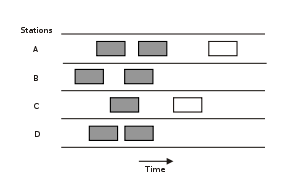
\includegraphics[width=1.2\textwidth]{pic/pure-aloha.png}
\end{block}
\column{.8\textwidth}
\begin{block}{Математическая модель}
\begin{itemize}
        \item Большое количество станций (чтобы пренебречь блокировкой станции), каждая генерирует редкий пуассоновский поток
        \item Суммарный поток заявок -- пуассоновский (передаем данные по мере поступления) с интенсивностью $\lambda$
        \item Все пакеты одинаковой длины $T = 1$
        \item Коллизии -- если есть пересечения во времени двух пакетов. При неудаче -- повтор.
\end{itemize}
\end{block}
\end{columns}
Пропускная способность канала -- максимальное количество успешно доставленных кадров в единицу времени в зависимости от нагрузки на канал ($N$ кадров за время кадра, $N < 1$)
\end{frame}
%--------------------------------------------------------------------------------
\begin{frame}
\frametitle{Пропускная способность ALOHA}
Пусть повторные попытки передачи также представляют собой пуассоновский поток. Старый кадры вместе с новыми создают пуассоновский поток интенсивностью $G\geq N$. При малой нагрузке $G\approx N$. Производительность канала равна
$$
S = GP_0, P_0\textrm{ -- вероятность успешной передачи кадра}
$$
Когда произойдет коллизия? Длина опасного интервала равна $2t$
\begin{center}
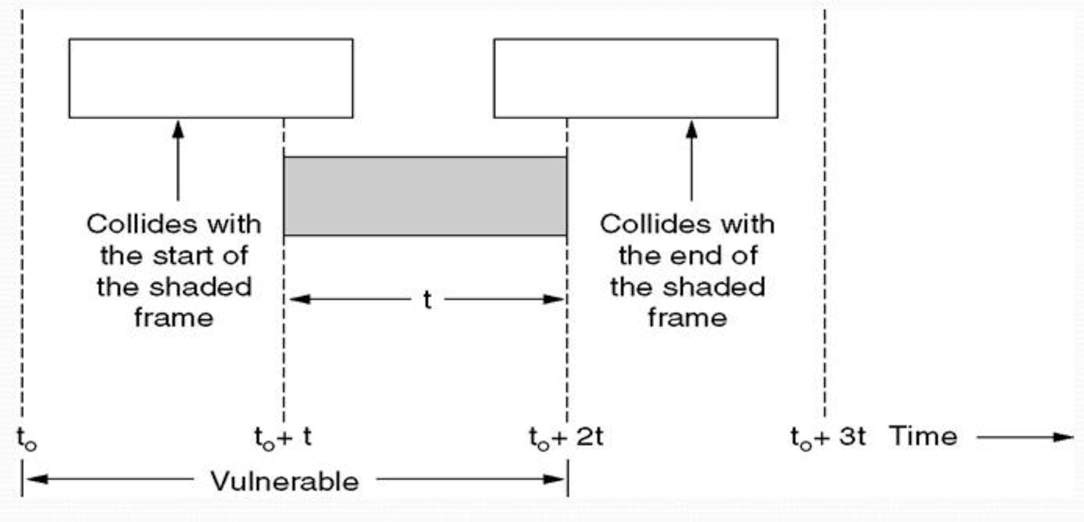
\includegraphics[width=0.6\textwidth]{pic/aloha-collision.pdf}
\end{center}
В течение опасного периода может начаться одна единственная передача!
\end{frame}
%--------------------------------------------------------------------------------
\begin{frame}
\frametitle{Пропускная способность ALOHA}
\begin{center}
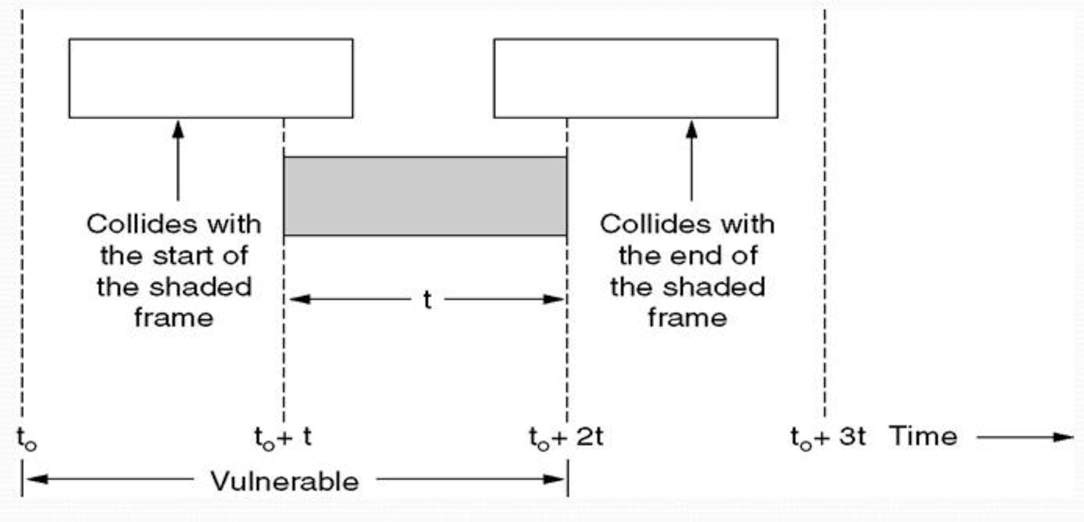
\includegraphics[width=0.45\textwidth]{pic/aloha-collision.pdf}
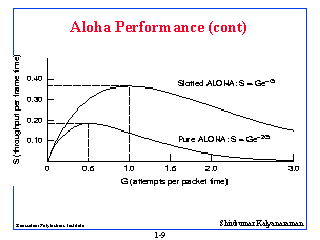
\includegraphics[width=0.32\textwidth]{pic/aloha-perf.png}
\end{center}
Вероятность того, что за время кадра будет сформировано $k$ кадров задается распределением Пуассона:
$$
Pr[k] = \frac{G^k e^{-G}}{k\!}
$$
Вероятность формирования нуля кадров за время кадра равно $e^{-G}$, нуля кадров за два времени кадра -- $e^{-2G}$. Итого:
$$
S = Ge^{-2G}, S_{max} = S_{G=0.5} = \frac{1}{2e}
$$
Производительность дискретной системы вдвое выше, достигается при единичной нагрузке.
\end{frame}
%--------------------------------------------------------------------------------
\begin{frame}
\frametitle{Пустые, успешные, коллизионные слоты в дискретной ALOHA}
Максимальная доля успешных слотов -- 37\%, доля пустых слотов -- 37\%, доля коллизионных - 26\%
Вероятность успеха с первой попытки равна $e^{-G}$, с $k$-ой --
$$
P_k = e^{-G} (1 - e^{-G})^k
$$
Ожидаемое число попыток передачи равно
$$
E = \sum_{k=1}^{+\infty}kP_k = \sum_{k=1}^{+\infty}ke^{-G} (1 - e^{-G})^k = e^G
$$
Количество повторных попыток передачи экспоненциально возрастает с нагрузкой.
\end{frame}
%--------------------------------------------------------------------------------
\begin{frame}
\frametitle{Протоколы с контролем несущей}
\begin{itemize}
\item Настойчивая CSMA -- передача с прослушиванием, случайное ожидание при коллизии. Чувствителен к задержкам на распространение сигнала (среда вроде бы свободна, но где-то ``вдалеке'' уже передают)
\item CSMA с настойчивостью $p$ -- снижение вероятности коллизии после длинного кадра. Случайное ожидание при коллизии
\item Ненастойчивая CSMA -- если при попытке начать передачу среда занята, то ожидаем случайное время.
\item CSMA/CD -- прекращение передачи при обнаружении коллизии (только проводные сети). Время обнаружения коллизии -- максимальное время распространения сигнала.
\end{itemize}
\end{frame}
%--------------------------------------------------------------------------------
\begin{frame}
\frametitle{Протоколы с контролем несущей}
\begin{center}
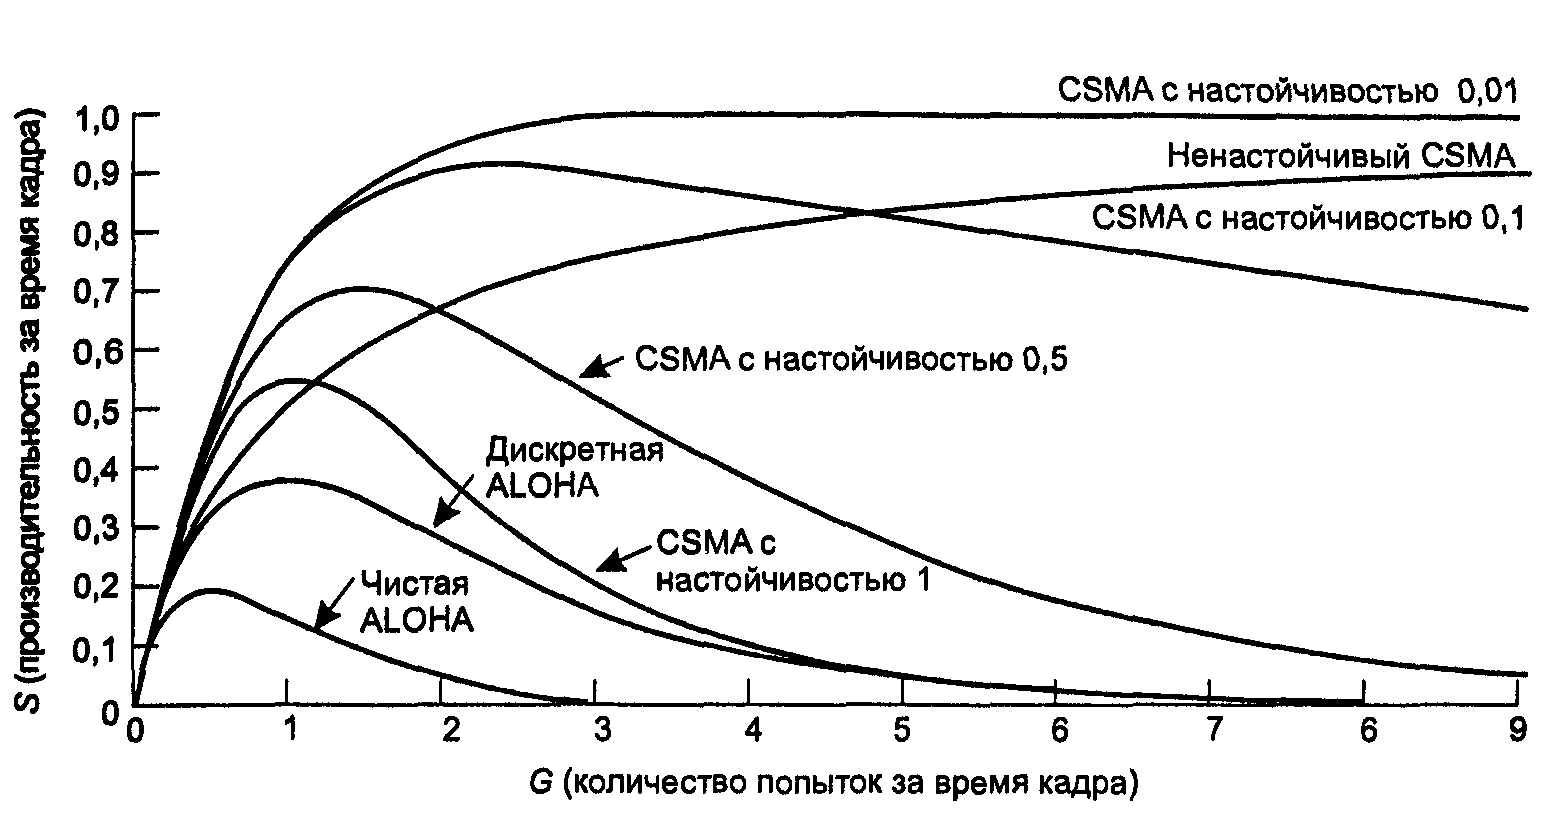
\includegraphics[width=\textwidth]{pic/csma-perf.png}
\end{center}
\end{frame}
%--------------------------------------------------------------------------------
\begin{frame}
\frametitle{Протоколы без столкновений}
\begin{itemize}
\item Протокол битовой карты: короткий кадр для передачи флага ``я передаю'', затем передают только те, кто имеет данные, по порядку
\item Двоичный обратный отсчёт: побитовое рассмотрение адреса желающих передать станций, выбывает тот, у кого ``0'' в текущем бите (DataKit)
\end{itemize}

\end{frame}
%--------------------------------------------------------------------------------
\begin{frame}
\frametitle{Протоколы с ограниченной конкуренцией}
\begin{itemize}
\item Отсутствие конкуренции ведет к высоким временам доставки данных, метод эффективнее при высоких нагрузках на сеть
\item Конкуренция снижает время доставки, однако метод доступа ведет к перегрузкам (снижение пропускной способности с ростом нагрузки)
\end{itemize}
\begin{itemize}
\item[*] Вероятность успешной передачи в дискретной системе из $k$ устройств при вероятности передачи каждого устройства в слоте $p$ составляет $kp(1-p)^{k-1}$, максимум при $p=\frac{1}{k}$
\item[*] Максимальная вероятность успеха равна $\Big(\frac{k-1}{k}\Big)^{k-1}$ -- быстро падает до $\frac{1}{e}$ с ростом $k$
\end{itemize}
Протокол адаптивного прохода по дереву -- все станции формируют листья двоичного дерева. Если произошла коллизия -- коллизионная группа уменьшается вдвое.
Начальная точка обхода дерева зависит от нагрузки.
\end{frame}
%--------------------------------------------------------------------------------
\begin{frame}
\frametitle{Особенности беспроводных сетей}
\begin{itemize}
\item Коллизию может распознать только приёмник
\item Проблема засвеченной станции
\item Проблема скрытой станции
\item CTS/RTS механизм -- Collision Avoidance
\end{itemize}
\end{frame}
%--------------------------------------------------------------------------------
\begin{frame}
 \frametitle{Физический уровень IEEE 802.11}
\begin{itemize}
 \item DSSS: Скорость передачи -- 1 МБод. Ширина спектра передаваемого сигнала -- 11 МГц. Скорость передачи -- 1МБит/с.
 \item FHSS: Смена рабочей частоты для снижения эффекта воздействия непреднамеренных помех
 \item OFDM: 64-FFT, используется 52 поднесущих, среди которых 4 -- пилотные
 \item HR-DSSS: Применяется в IEEE 802.11b. Скорости передачи до 11 МБит/с.
\end{itemize}
\end{frame}
%--------------------------------------------------------------------------------
\begin{frame}
\frametitle{Режимы работы сети IEEE 802.11}
\begin{itemize}
 \item Инфраструктурный, предполагающий наличие базовой станции (Access Point)
 \begin{itemize}
  \item Ассоциация и аутентификация
  \item Распределённый доступ к среде
  \item Координированный доступ к среде
  \item Обеспечение качества обслуживания
 \end{itemize}
 \item Распределённый режим
 \item Многошаговый режим (IEEE 802.11s)
\end{itemize}
\end{frame}
%--------------------------------------------------------------------------------
\begin{frame}
\frametitle{Механизмы доступа к среде в IEEE 802.11}
\begin{itemize}
 \item Время разделено на временные слоты
 \item Случайный множественный доступ с предотвращением коллизий
 \item Определение занятости среды
 \begin{enumerate}
  \item Фактическая занятость среды
  \item Виртуальная занятость среды
 \end{enumerate}

 \item Детерминированный множественный доступ (только инфраструктурный режим)
 \item Механизм двоичного экспоненциального отката
\end{itemize}
\end{frame}
%--------------------------------------------------------------------------------
\begin{frame}
\frametitle{Структура кадра IEEE 802.11}
\begin{center}
 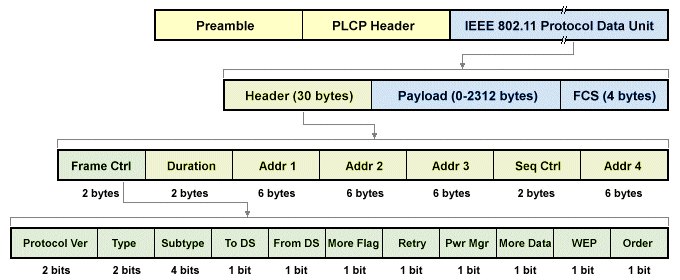
\includegraphics[width=\textwidth]{pic/802-11-frame.png}
\end{center}
\end{frame}
%--------------------------------------------------------------------------------
\begin{frame}
\frametitle{Механизм доступа к среде IEEE 802.11}
\begin{center}
 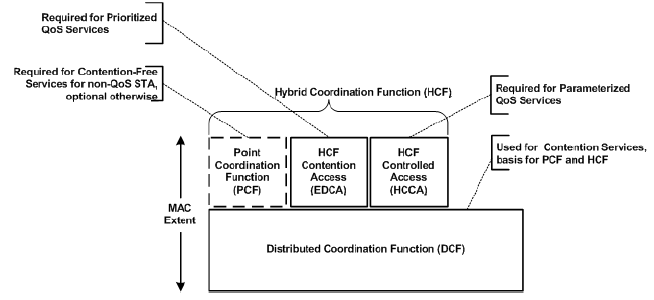
\includegraphics[width=\textwidth]{pic/802-11-dcf.png}
\end{center}
\end{frame}
%--------------------------------------------------------------------------------
\begin{frame}
\frametitle{Структура межфреймовых интервалов}
\begin{center}
 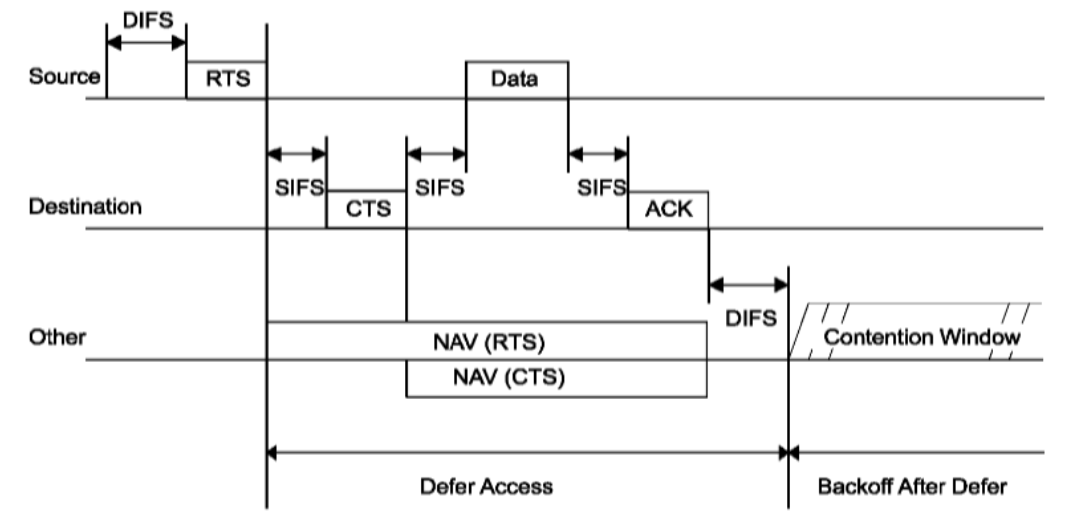
\includegraphics[width=\textwidth]{pic/ifs-structure.png}
\end{center}
\end{frame}
%--------------------------------------------------------------------------------
\begin{frame}
\frametitle{Случайный множественный доступ с обеспечением приоритетов}
\begin{center}
 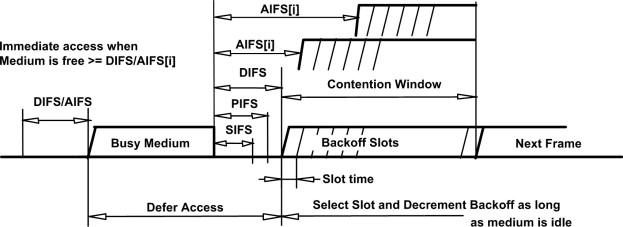
\includegraphics[width=\textwidth]{pic/802-11-ifs.png}
\end{center}
\begin{itemize}
 \item [+] получение грантов на передачу (TXOP)
\end{itemize}
\end{frame}
%--------------------------------------------------------------------------------
\begin{frame}
\frametitle{Очереди с приоритетом и внутренним разрешением коллизий}
\begin{center}
 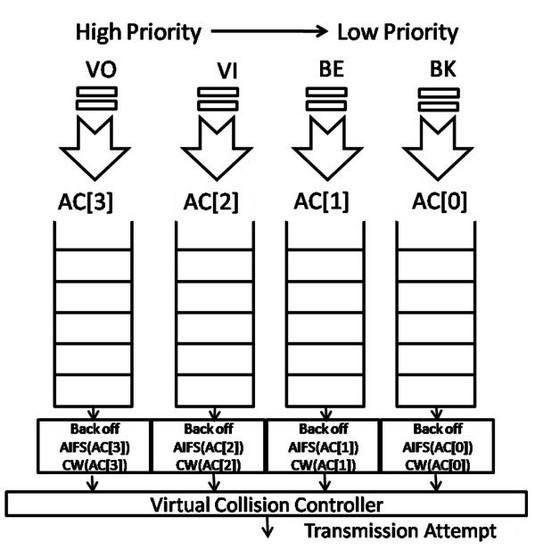
\includegraphics[width=0.6\textwidth]{pic/edca.png}
\end{center}
\end{frame}
%--------------------------------------------------------------------------------
\begin{frame}
\frametitle{Дифференциация поступающих данных на классы}
\begin{center}
 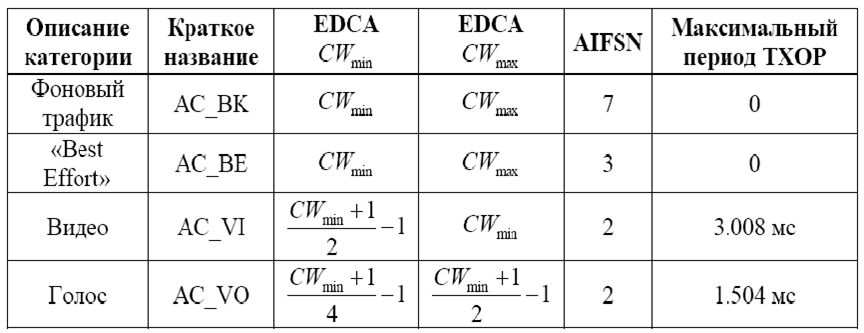
\includegraphics[width=\textwidth]{pic/access-classes.png}
\end{center}
\end{frame}
%--------------------------------------------------------------------------------
\begin{frame}
\frametitle{Заморозка счётчика отсрочки}
\begin{center}
 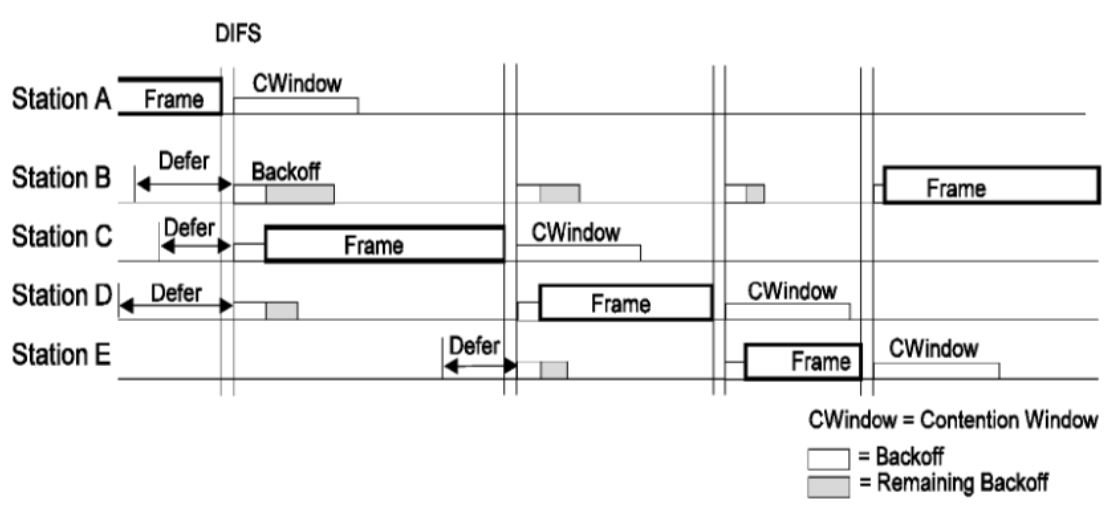
\includegraphics[width=\textwidth]{pic/backoff.png}
\end{center}
\end{frame}
%--------------------------------------------------------------------------------
\begin{frame}
\frametitle{CTS/RTS и потеря кадра}
\begin{center}
 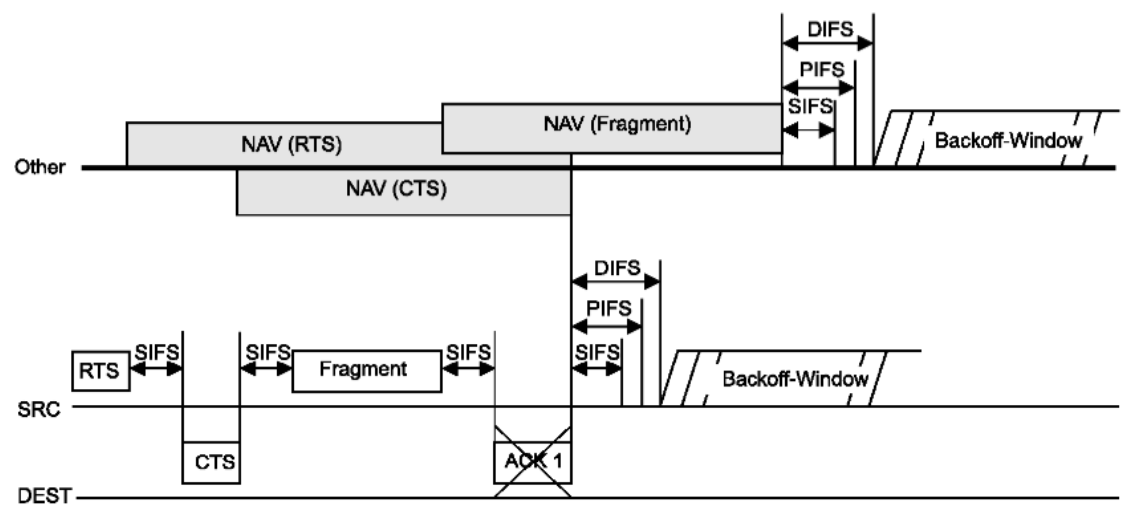
\includegraphics[width=\textwidth]{pic/cts-rts.png}
\end{center}
\end{frame}
%--------------------------------------------------------------------------------
\begin{frame}
 \frametitle{Работа в инфраструктурном режиме}
\begin{itemize}
 \item Периодическая высокоприоритетная рассылка служебной информации (beacon)
 \item Механизм аутентификации
 \item Механизм ассоциации (Association request/response)
 \item Контролируемый доступ к среде
\end{itemize}
\begin{block}{Работа AP в PCF -- Point Coordination Function}
\begin{itemize}
 \item AP имеет список всех ассоциированных клиентов и список опроса
 \item Передача от AP возможна в любой момент спустя SIFS после beacon и успешной передачи, PIFS после потери кадра
 \item Передача к AP возможна только после опроса CF-Poll, и только однократная передача
\end{itemize}
\end{block}

\end{frame}

%--------------------------------------------------------------------------------
%--------------------------------------------------------------------------------
\begin{frame}
\frametitle{Инфраструктурный режим}
\begin{center}
 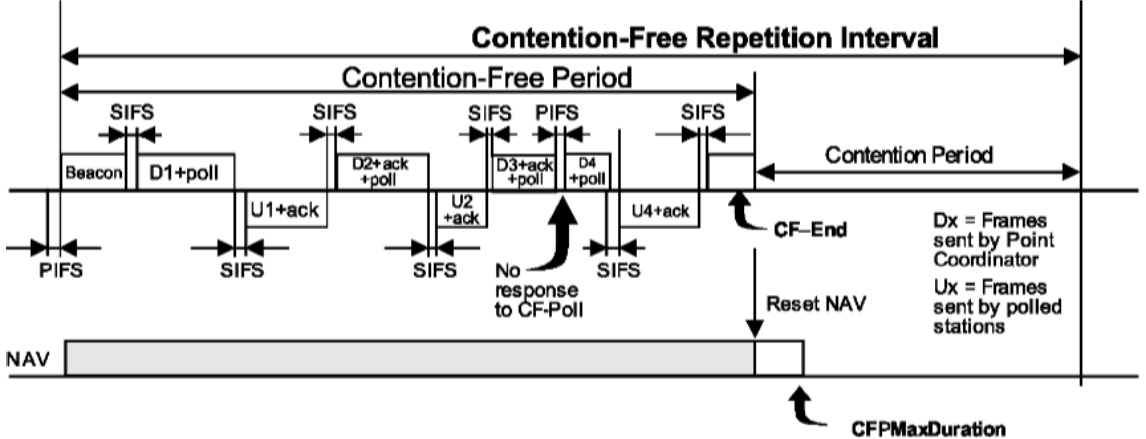
\includegraphics[width=\textwidth]{pic/pcf.png}
\end{center}
\end{frame}
%--------------------------------------------------------------------------------
%--------------------------------------------------------------------------------
%--------------------------------------------------------------------------------
\begin{frame}
\frametitle{Механизмы адаптации канальной скорости}
\begin{itemize}
 \item Переменные свойства беспроводного канала
 \item Необходимость достижения максимальной пропускной способности
 \item Различные варианты модуляции и кодовых скоростей
\end{itemize}
Необходимость управления канальной скоростью передачи (выбором модуляции и кодовой скорости)
\begin{block}{Minstrel -- Multi Rate Retry}
\begin{enumerate}
 \item ``Пробные пакеты'', выбираемые для оценки канала для всех скоростей
 \item Вычисление скорости с наибольшей пропускной способностью
 \item Вычисление скорости с наилучшей вероятностью успешной доставки пакета
 \item Использование фильтров при обработке статистики (EWMA)
\end{enumerate}
\end{block}
\end{frame}
%--------------------------------------------------------------------------------
\begin{frame}
\frametitle {Политика повторов в алгоритме Minstrel}
\begin{center}
 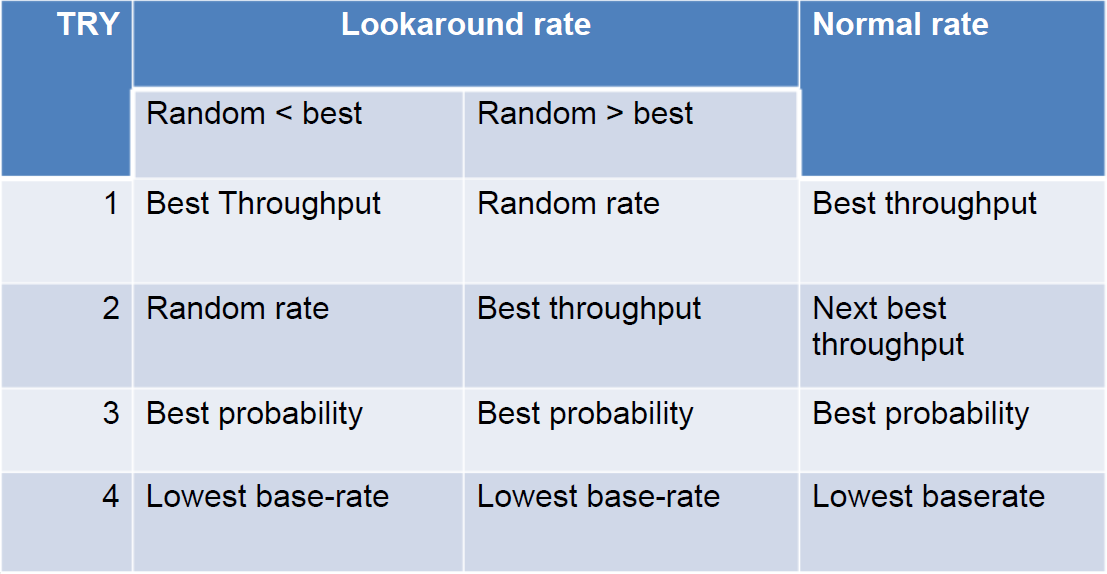
\includegraphics[width=\textwidth]{pic/minstrel.png}
\end{center}
\end{frame}
%--------------------------------------------------------------------------------
\begin{frame}
\frametitle{Режим блочной передачи}
\begin{center}
 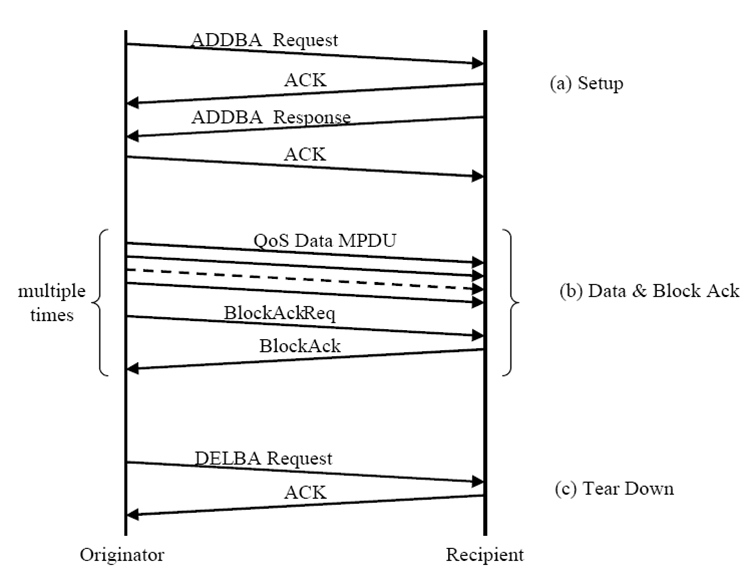
\includegraphics[width=\textwidth]{pic/bloack-ack.png}
\end{center}
\end{frame}
%--------------------------------------------------------------------------------
\begin{frame}
\frametitle{Механизмы блочных подтверждений}
\begin{block}{Механизмы подтверждений}
 \begin{itemize}
  \item Отсутствие подтверждений
  \item Мгновенное подтверждение
  \item Подтверждение с задержкой
 \end{itemize}
\end{block}
\begin{block}{Типы блочных подтверждений}
 \begin{itemize}
  \item Мгновенные
  \item С задержкой
 \end{itemize}
\end{block}
\end{frame}
%--------------------------------------------------------------------------------
\begin{frame}
\frametitle{Immediate Block ACK}
\begin{center}
 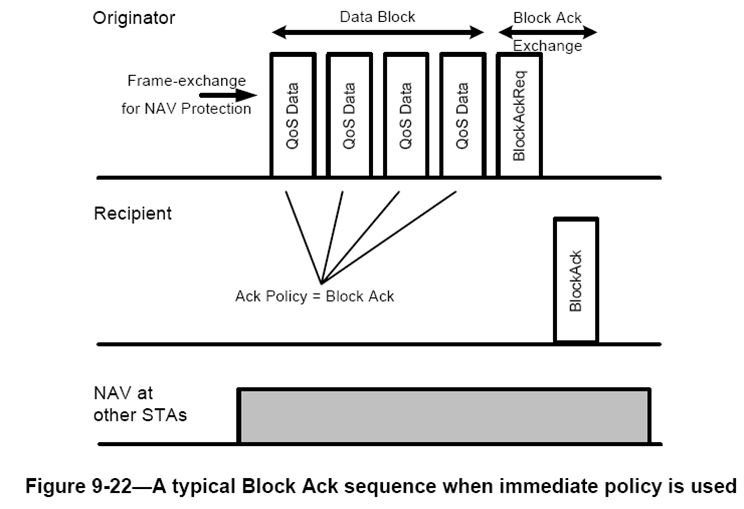
\includegraphics[width=\textwidth]{pic/immediate-block-ack.png}
\end{center}
\end{frame}
%--------------------------------------------------------------------------------
\begin{frame}
\frametitle{Delayed Block ACK}
\begin{center}
 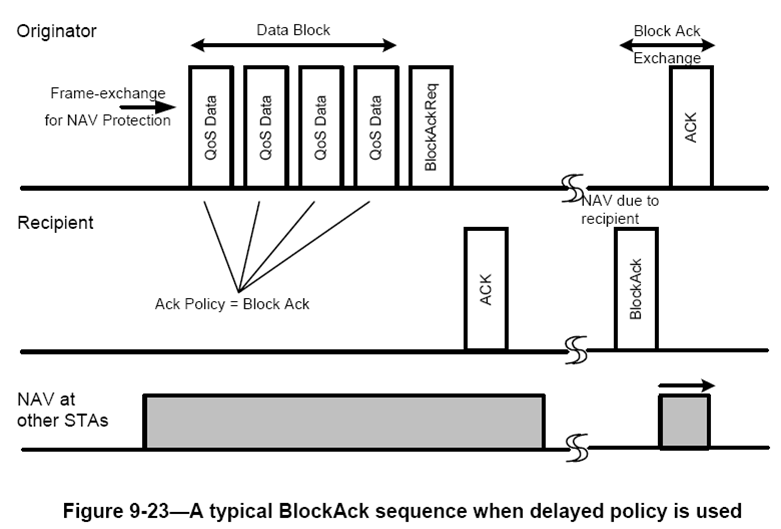
\includegraphics[width=\textwidth]{pic/delayed-block-ack.png}
\end{center}
\end{frame}
%--------------------------------------------------------------------------------
\end {document}
